\section*{Interfaces para el sonido}

\item
\begin{minipage}[t][2.8cm]{0.6\textwidth}
Como nos interesa estudiar la unión de dos caños cuadrados de área transversal $A_1$ y $A_2$ los consideramos semi--infinitos.
Desde el izquierdo incide una onda acústica $\delta p_i (x,t) = a_i \cos{ \left( k_i x - \omega t \right) }$.
Suponga despreciables los efectos de la viscosidad y dé por conocidos $A_{1}$, $A_{2}$, presión media $P_{0}$, densidad media $\rho_{0}$, $v_{s}$, $\omega$, $a_i$.
Halle amplitudes de presión y desplazamiento de moléculas a causa de las ondas reflejadas y transmitidas.
\end{minipage}
\begin{minipage}[c][0cm][t]{0.34\textwidth}
	\includegraphics[width=\textwidth]{ej2-10}
\end{minipage}



\item 
\begin{minipage}[t][1.4cm]{0.6\textwidth}
A este armado con idénticas áreas del problema anterior incide la misma onda.
Halle $\delta p(x,t)$ y $\psi(x,t)$ en cada tramo.
\end{minipage}
\begin{minipage}[c][1.4cm][t]{0.34\textwidth}
	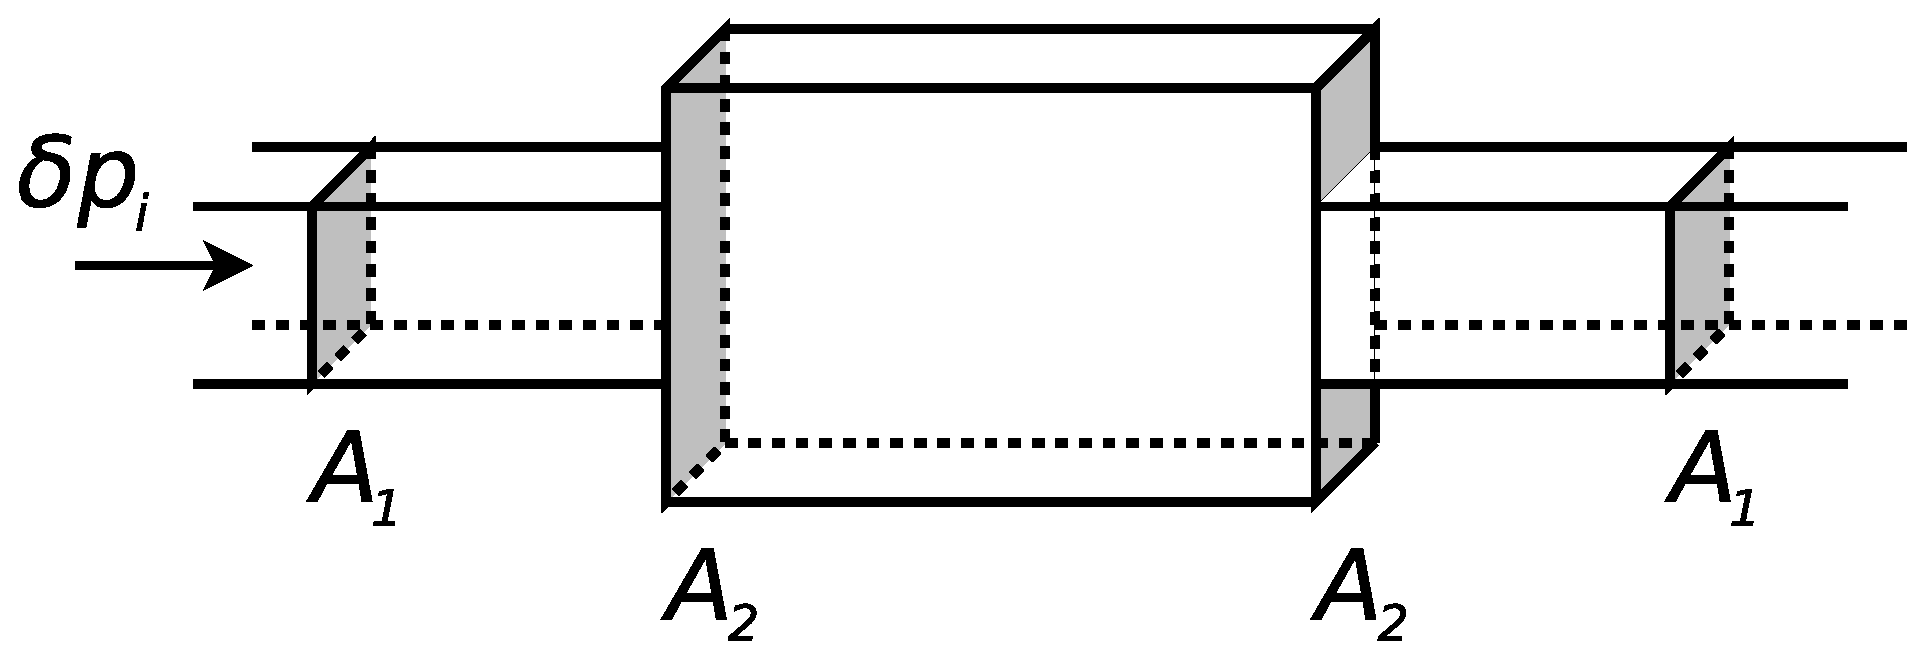
\includegraphics[width=\textwidth]{ej2-11}
\end{minipage}



\item
\begin{minipage}[t][1.6cm]{0.75\textwidth}
(*) Desde el aire incide en dirección perpendicular a una superficie calma de agua una onda de sonido plana $\delta p_i (y,t) = A_i \cos{\left( k_i y - \omega t \right)}$.
Hallar la onda reflejada $\delta p_{r}(y,t)$ y transmitida $\delta p_{t}(y,t)$.
\end{minipage}
\begin{minipage}[c][0.8cm][t]{0.2\textwidth}
	\includegraphics[width=\textwidth]{ej2-12}
\end{minipage}
%\begin{figure}[ht]
%\centering{}\includegraphics[clip,scale=0.25]{ej2-12}
%\end{figure}


\item (*)
Calcule los coeficientes de reflexión y de transmisión del sonido en las siguientes interfases:\\
\begin{enumerate*}[label=\alph*),itemjoin={,\quad}]
	\item Fe-Cu
	\item Al-Pb
\end{enumerate*}
%\begin{enumerate}
%	\item Fe-Cu
%	\item Al-Pb
%\end{enumerate}


\end{enumerate}

\end{document}
